\documentclass[international_finance_p1.tex]{subfiles}

\begin{document}
\setbeamercovered{transparent}
\section{International Monetary Arrangements}
\subsection{The Gold Standard and Interwar Period}
\begin{frame}{The Gold Standard: 1880 to 1914. The Interwar Period: 1918 to 1939}
\begin{itemize}[<+->]
\item
Under a gold standard, currencies are valued in terms of their gold equivalent (an ounce of gold was worth USD20.67 in terms of the U.S. dollar over the gold standard period). 
\item
The I World War ended Britain’s financial preeminence.
\item
The United States had risen to the status of the world’s dominant banker country.
\end{itemize}
\end{frame}
\begin{frame}{}
% Table generated by Excel2LaTeX from sheet 'Лист1'
\begin{table}[htbp]
  \centering
  \fontsize{6pt}{6pt}\selectfont
  \caption{Leading central bank/treasury gold reserves(in metric tons fine gold)}
    \begin{tabular}{lrrrrrrrr}
    \toprule
    Year  & 1845  & 1850  & 1855  & 1860  & 1865  & 1870  & 1875  & 1880 \\
  \midrule
UK    & 82    & 104   & 74    & 78    & 93    & 161   & 154   & 170 \\
    France & 2     & 3,5   & 32,8  & 105   & 194   & 217   & 337   & 242 \\
    Germany & n/a   & n/a   & n/a   & n/a   & n/a   & n/a   & 43    & 81 \\
    Italy & n/a   & n/a   & n/a   & n/a   & n/a   & 30,8  & 26    & 22 \\
    Russia & n/a   & n/a   & 81    & n/a   & 57    & 160   & 230   & 195 \\
    USA   & n/a   & n/a   & n/a   & n/a   & n/a   & 107   & 87    & 208 \\
    \bottomrule
    \end{tabular}%
  \label{tab:addlabel}%

\raggedright
\footnotesize
Source: World Gold Council. Historical Data - Annual time series on 
World Official Gold Reserves since 1845. 10th August 2011.
\end{table}%
\end{frame}

\begin{frame}
% Table generated by Excel2LaTeX from sheet 'Лист1'
\begin{table}[htbp]
  \centering
  \fontsize{6pt}{6pt}\selectfont
  \caption{Leading central bank/treasury gold reserves(in metric tons fine gold)}
    \begin{tabular}{lrrrrrrrr}
    \toprule
    Year  & 1885  & 1890  & 1895  & 1900  & 1905  & 1910  & 1913  & 1915 \\
    \midrule
UK    & 141   & 166   & 305   & 198   & 199   & 223   & 248   & 585 \\
    France & 344   & 370   & 460   & 544   & 836   & 952   & 1030  & 1457 \\
    Germany & 99    & 186   & 252   & 211   & 267   & 240   & 437   & 876 \\
    Italy & 142   & 133   & 132   & 115   & 285   & 350   & 355   & 397 \\
    Russia & 195   & 312   & 695   & 661   & 654   & 954   & 1233  & 1250 \\
    USA   & 371   & 442   & 169   & 602   & 1149  & 1660  & 2293  & 2568 \\
    \bottomrule
    \end{tabular}%
  \label{tab:addlabel}%

\raggedright
\footnotesize
Source: World Gold Council. Historical Data - Annual time series on 
World Official Gold Reserves since 1845. 10th August 2011.
\end{table}%

\end{frame}

\begin{frame}
% Table generated by Excel2LaTeX from sheet 'Лист1'
\begin{table}[htbp]
  \centering
  \fontsize{6pt}{6pt}\selectfont
  \caption{Leading central bank/treasury gold reserves(in metric tons fine gold)}
    \begin{tabular}{lrrrrrr}
    \toprule
    Year  & 1920  & 1925  & 1930  & 1935  & 1940  & 1945 \\
    \midrule
UK    & 864   & 1045  & 1080  & 1464  & n/a   & 1773 \\
    France & 1622  & 1201  & 3160  & 3907  & 1773  & 1378 \\
    Germany & 391   & 432   & 794   & 56    & n/a   & n/a \\
    Italy & 307   & 498   & 420   & 240   & 122   & 28 \\
    Russia & n/a   & 141   & 375   & 7456  & n/a   & n/a \\
    USA   & 3679  & 5998  & 6358  & 8998  & 19543 & 17848 \\
    \bottomrule
    \end{tabular}%
  \label{tab:addlabel}%

\raggedright
\footnotesize
Source: World Gold Council. Historical Data - Annual time series on 
World Official Gold Reserves since 1845. 10th August 2011.
\end{table}%
\end{frame}

\begin{frame}{}
\begin{itemize}[<+->]
\item
So a run on U.S. gold at the end of 1931 led to a 15 percent drop in U.S. gold holdings. By 1933 the United States abandoned the gold standard.
\item
The early to mid-1930s was a period of competitive devaluations and foreign exchange controls.
\end{itemize}
\end{frame}
\subsection{The Bretton Woods Agreement}
\begin{frame}{The Bretton Woods Agreement: 1944 to 1973 and its breakdown}
\begin{itemize}[<+->]
\item
Bretton Woods agreement required each country to fix the value of its currency in terms of an anchor currency, namely the dollar. 
\item
The U.S. dollar was the key currency in the system, and USD1 was defined as being equal in value to 1/35 ounce of gold. 
\item
Since every currency had an implicitly defined gold value, through the link to the dollar, all currencies were linked in a system of fixed exchange rates.
\end{itemize}
\end{frame}
\begin{frame}{}
\begin{itemize}[<+->]
\item
Nations were committed to maintaining the parity value of their currencies within 1 percent of parity. 
\item
When a country was experiencing difficulty maintaining its parity value because of balance of payments disequilibrium, it could turn to the International Monetary Fund (IMF).
\end{itemize}
\end{frame}
\begin{frame}{}
\begin{itemize}[<+->]
\item
The IMF was created to monitor the operation of the system and provide short-term loans to countries experiencing temporary balance of payments difficulties. 
\item
IMF conditions for loans were changes in domestic economic policy aimed at restoring balance of payments equilibrium.
\end{itemize}
\end{frame}
\begin{frame}{}
\begin{itemize}[<+->]
\item
The failure to realign currency values in the face of fundamental economic change spelled the beginning of the end for the gold exchange standard of the Bretton Woods agreement by the late 1960s.
\item
In December 1971, the dollar per gold exchange value was changed from USD35 to USD38.02 per ounce of gold. But the dollar was still inconvertible into gold.
\item
The speculative capital flows of 1972 and early 1973 led to a further devaluation of the dollar in February 1973, when the official price of an ounce of gold rose from USD38 to USD42.22.
\item
In March 1973, the major currencies began to float
\end{itemize}
\end{frame}
\subsection{Floating Exchange Rates}
\begin{frame}{Floating Exchange Rates: starting from 1973}
The types of exchange rate systems

1. Free floating. 

2. Managed floating.

3. Horizontal bands.

4. Crawling pegs. 

5. Crawling bands.

6. Fixed peg. 

7. Currency board. 

8. ``Dollarization'' or No separate legal tender.
\end{frame}
\begin{frame}{}
\begin{itemize}[<+->]
\item
\textbf{“dollarization” }where the central bank of the country has completely given up control of the money supply to adopt some other country’s currency
\item
\textbf{purely floating}, where the central bank retains domestic control over the currency in the country. 
\item
In between, the central bank has some degree of control over the money supply.
\end{itemize}
\end{frame}
\begin{frame}{What is ``Legal Tender''}
\begin{block}{Legal tender }
\quad is any official medium of payment recognized by law that can be used to extinguish a public or private debt, or meet a financial obligation. The national currency is legal tender in practically every country. A creditor is obligated to accept legal tender toward repayment of a debt. Legal tender can only be issued by the national body that is authorized to do so, such as the U.S. Treasury in the United States and the Royal Canadian Mint in Canada.
\end{block}
The term "legal tender" is from Middle English tendren, French tendre (verb form), meaning to offer. The Latin root is tendere (to stretch out), and the sense of tender as an offer is related to the etymology of the English word "extend" (to hold outward).
\end{frame}
\begin{frame}{What does ``Tender'' mean}
\begin{block}{To tender}
To invite bids for a project, or to accept a formal offer such as a takeover bid. Tender usually refers to the process whereby governments and financial institutions invite bids for large projects that must be submitted within a finite deadline. The term also refers to the process whereby shareholders submit their shares or securities to a takeover offer.
\end{block}
\end{frame}
\begin{frame}{Legal Tender and Standard of Deferred Payment}
A debt is a deferred payment; a standard of deferred payment is what they are denominated in. 

Since the value of money – be it dollars, gold, or others – may fluctuate over time via inflation and deflation, the value of deferred payments (the real level of debt) likewise fluctuates. 

A device is termed ``legal tender'' if it may serve to discharge (pay off) debts; thus, while US dollars are not backed by gold or any other commodity, they draw value from being legal tender – being usable to pay off debts.
\end{frame}
\begin{frame}{Characteristics Associated with Countries Choosing to Peg or Float}
% Table generated by Excel2LaTeX from sheet 'Лист2'
\begin{table}[htbp]
  \centering
    \begin{tabular}{cc}
    \toprule
    Peggers & Floaters \\
    \midrule
    Small size & Large size  \\
    Open economy & Closed economy  \\
    Harmonious inflation rate  & Divergent inflation rate \\
    Concentrated trade  & Diversified trade \\
    \bottomrule
    \end{tabular}%
  \label{tab:addlabel}%
\end{table}%
\end{frame}
\subsection{Plaza and Louvre Accord}
\begin{frame}{Plaza Accord}
\begin{itemize}[<+->]
\item
Between 1980 and 1985 the dollar had appreciated by about 50\% against the Japanese yen, Deutsche Mark, French Franc and British pound
\item
Campaign asking for protection against foreign competition
\item
The governments of France, West Germany, Japan, the United States, and the United Kingdom signed the accord to depreciate the U.S. dollar in relation to the Japanese yen and German Deutsche Mark by intervening in currency markets on September 22, 1985 at the Plaza Hotel in New York City.
\item
The exchange rate value of the dollar versus the yen declined by 51\% from 1985 to 1987.
\end{itemize}
\end{frame}
\begin{frame}{Louvre Accord}
\begin{itemize}[<+->]
\item
The Louvre Accord was an agreement, signed on February 22, 1987 in Paris, that aimed to stabilize the international currency markets and halt the continued decline of the US Dollar caused by the Plaza Accord.
\item
The Louvre Accord helped prevent a recession because it stopped the value of the U.S. Dollar from decreasing any further in relation to other currencies.
\item
Countries agreed to reduce budget deficits and government spendings, cut taxes, USA agreed to hold interest rates low.
\end{itemize}
\end{frame}

\subsection{The European Monetary System}
\begin{frame}{The European Monetary System and the Euro}
\begin{itemize}[<+->]
\item
The European Monetary System (EMS) was established in March 1979. 
\item
The member countries agreed to maintain small exchange rate fluctuations among themselves, while allowing free float against outside currencies.

\end{itemize}
\end{frame}
\begin{frame}{The theory of optimum currency area}
{Professor Robert Mundell of Columbia University, 1961}
\begin{block}{Criterion for a common currency zone }
The relevant criterion for identifying and designing a common currency zone is the degree of factor (i.e., capital and labor) mobility within the zone; a high degree of factor mobility would provide an adjustment mechanism, providing an alternative to country-specific monetary/currency adjustments.
\end{block}
\end{frame}

\begin{frame}[shrink=15]{Monetary Unions I}
% Table generated by Excel2LaTeX from sheet 'Лист2'
\begin{table}[htbp]
  \centering
    \begin{tabular}{ll}
    \toprule
    \multicolumn{1}{c}{Monetary union} & \multicolumn{1}{c}{Participants} \\
    \midrule
    \pbox{3cm}{European Union (EU)} & \pbox{6cm}{Austria, Belgium, Bulgaria, Cyprus, Czech Republic, Germany, Denmark, Spain, Estonia, Finland, France, United Kingdom, Greece, Croatia, Hungary, Ireland, Italy, Lithuania, Luxembourg, Latvia, Malta, Netherlands, Poland, Portugal, Romania, Slovakia, Slovenia, Sweden}  \\
    \midrule
    \pbox{3cm}{Commonwealth of \\Independent States (CIS)} & \pbox{6cm}{Armenia, Azerbaijan, Belarus, Kazakhstan, Kyrgyzstan, Moldova, Russia, Tajikistan, Uzbekistan} \\
    \midrule
    \pbox{3cm}{Asian Monetary Unit (AMU)} & \pbox{6cm}{Australia, Brunei, China, Indonesia, India, Japan, Cambodia, South Korea, Laos, Myanmar, Malaysia, New Zealand, Philippines, Singapore, Thailand, Vietnam} \\
    \bottomrule
    \end{tabular}%
  \label{tab:addlabel}%
\end{table}%
\end{frame}

\begin{frame}[shrink=10]{Monetary Unions II}
% Table generated by Excel2LaTeX from sheet 'Лист2'
\begin{table}[htbp]
  \centering
    \begin{tabular}{ll}
    \toprule
    \multicolumn{1}{c}{Monetary union} & \multicolumn{1}{c}{Participants} \\
    \midrule
    \pbox{4cm}{East African Community (EAC)} & \pbox{5cm}{Burundi, Kenya, Rwanda, Tanzania, Uganda} \\
    \midrule
    \pbox{4cm}{Economic Community of \\West African States (Ecowas)} & \pbox{5cm}{Benin, Burkina Faso, CapeVerde, Gambia, Ghana, Guinea, Guinea-Bissau, Ivory Coast, Liberia, Mali, Niger, Nigeria, Senegal, Sierra Leone, Togo} \\
    \midrule
    \pbox{4cm}{Bolivarian Alliance for the Peoples of Our America (AlBA)} & \pbox{5cm}{Antigua and Barbuda, Bolivia, Cuba, Dominica, Ecuador, Grenada, Saint Kitts and Nevis, Saint Lucia, Nicaragua, Saint Vincent and the Grenadines, Venezuela} \\
    \bottomrule
    \end{tabular}%
  \label{tab:addlabel}%
\end{table}%
\end{frame}

\begin{frame}{Existing and emerging monetary unions}
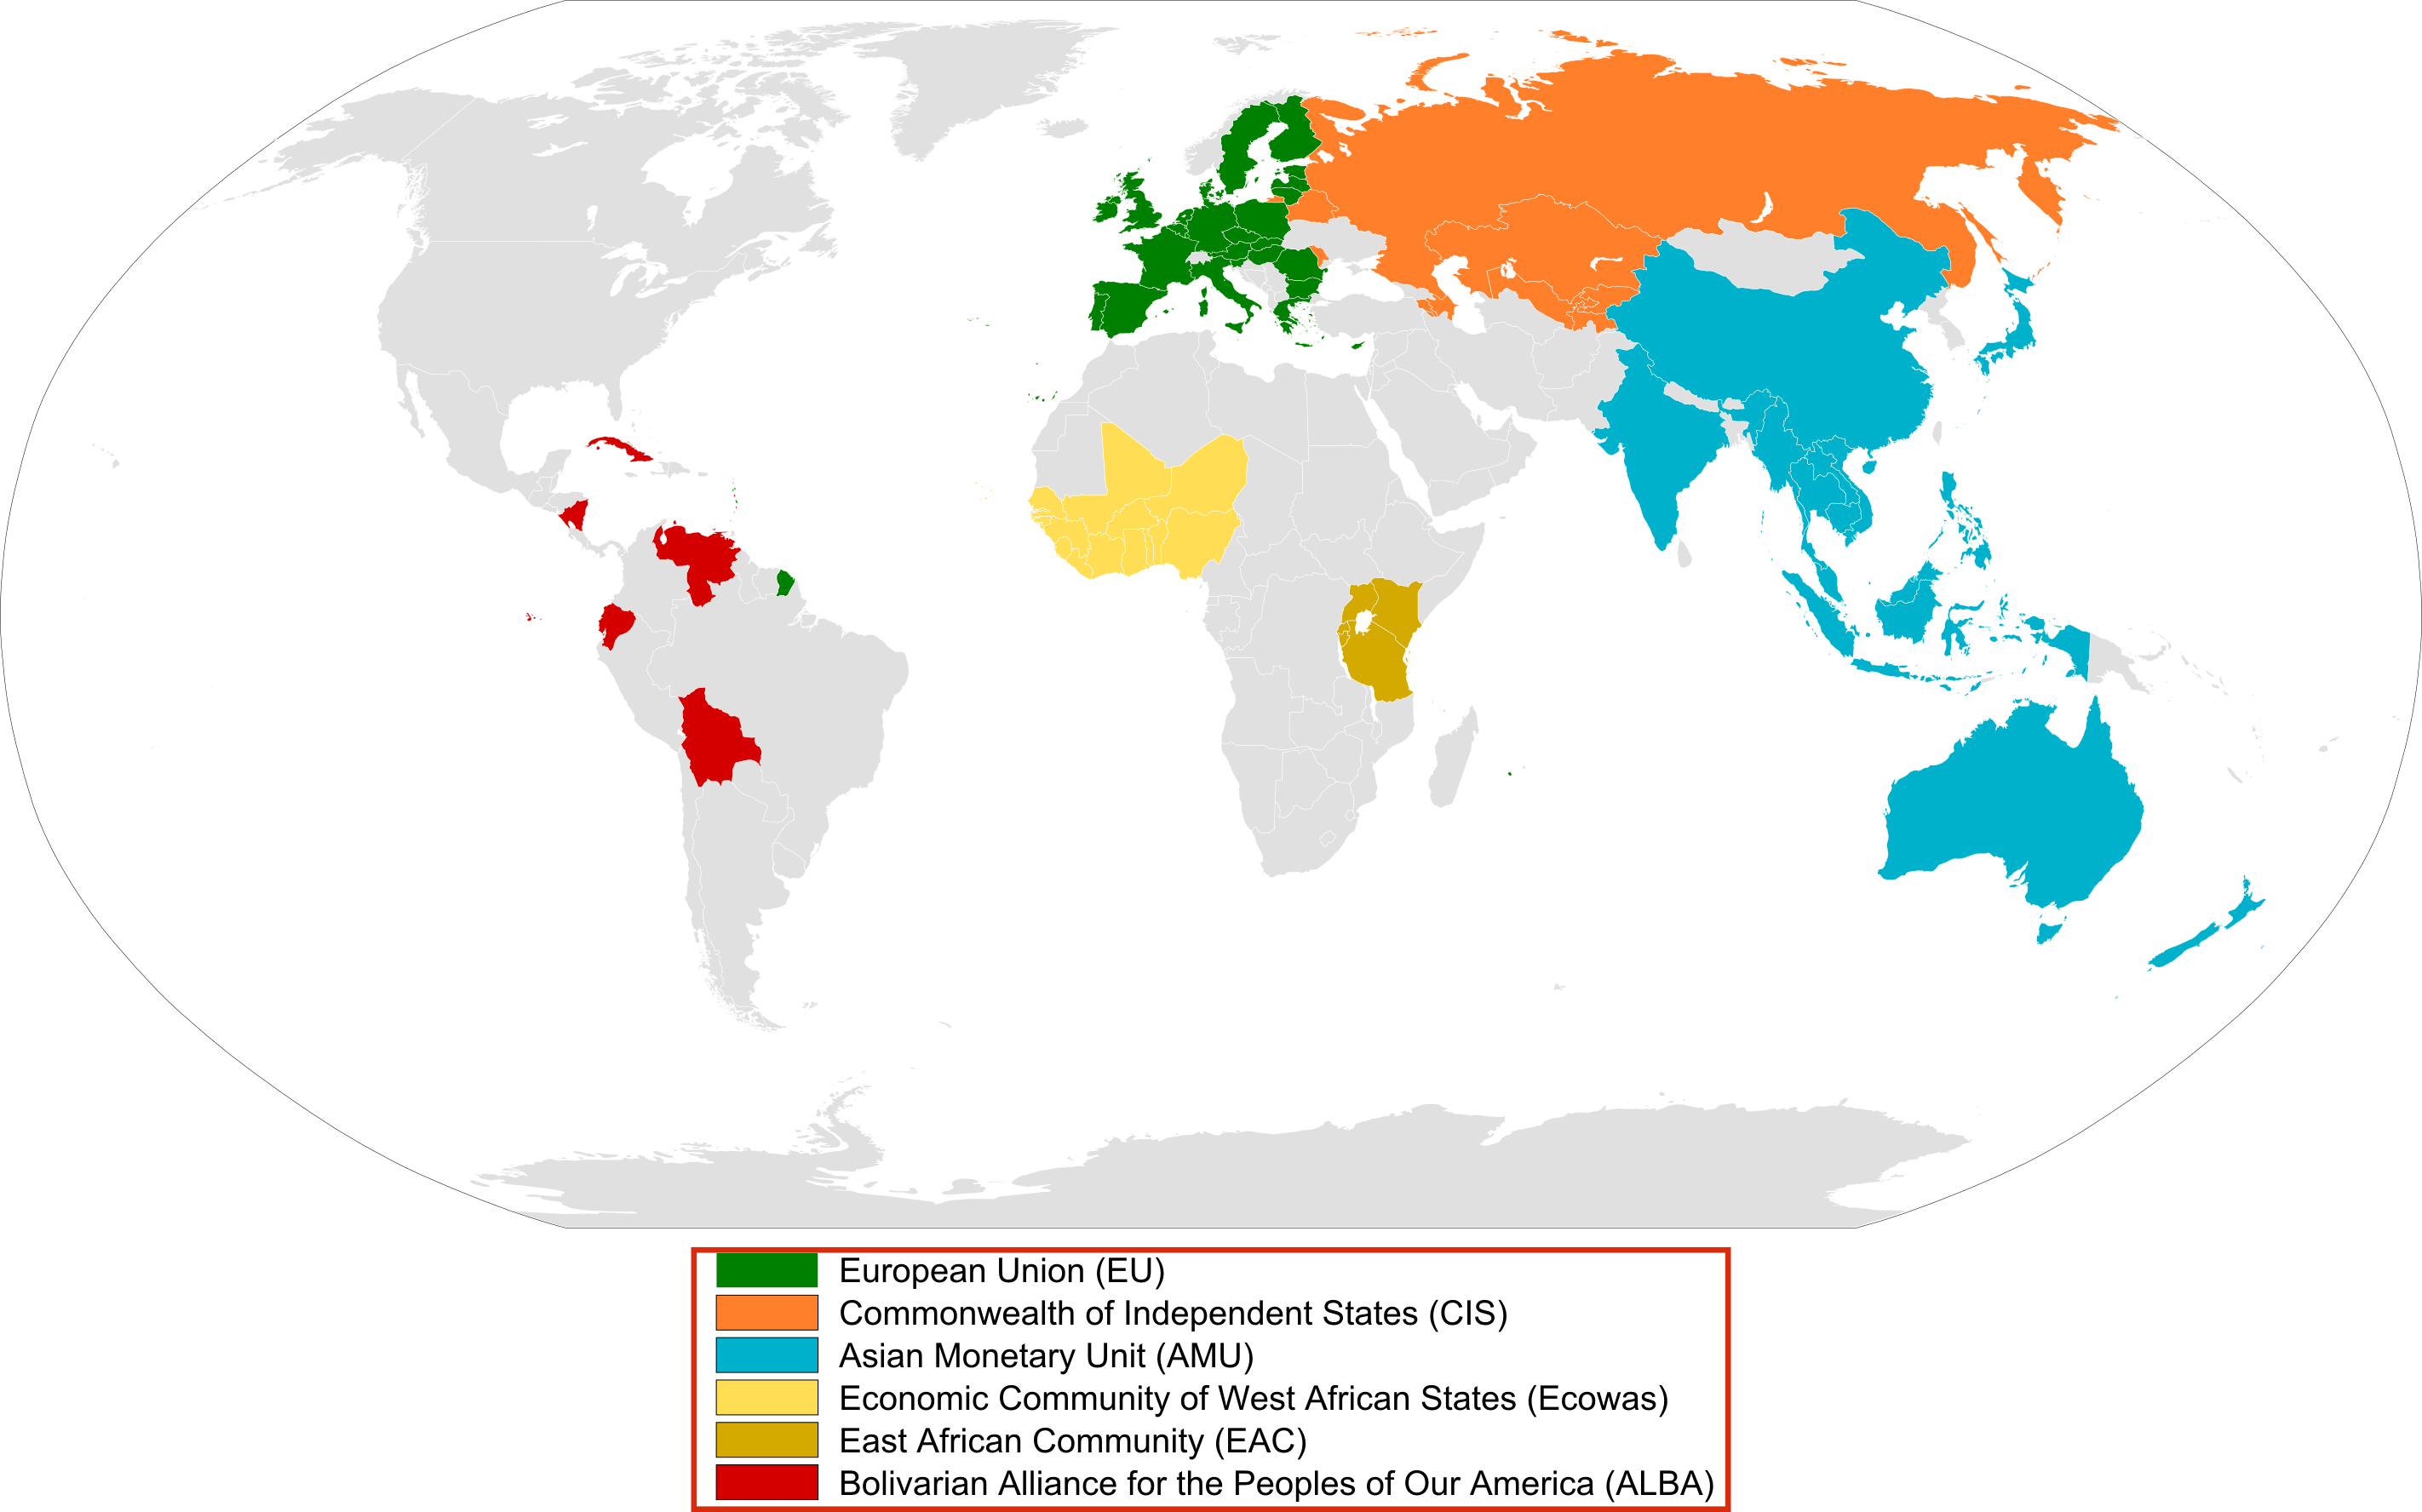
\includegraphics[scale=0.40]{img/monetaryunions}
\end{frame}

\begin{frame}{Convergence of monetary policy}
\begin{itemize}[<+->]
\item
the country’s inflation rate did not exceed the average of the lowest three member country rates by more than 1.5 percentage points; 
\item
its interest rate on long-term government bonds did not exceed those of the three lowest-inflation members by more than 2 percentage points; 
\item
the country’s government budget deficit did not exceed 3 percent of GDP, and outstanding government debt did not exceed 60 percent of GDP.
\end{itemize}
\end{frame}

\begin{frame}{The optimum currency area}
\begin{itemize}[<+->]
\item
The geographical region that could gain economic efficiency by fixing exchange rates within a group and floating exchange rates with the rest of the world. 
\item
Necessary condition is perfect mobility of the factors of production.
\end{itemize}
\end{frame}

\begin{frame}{The European Central Bank (ECB)}
\begin{itemize}[<+->]
\item
Created on June 1, 1998, in Frankfurt, Germany. 
\item
The European Central Bank (ECB) is responsible for monetary policy of the Eurozone. 
\item
The ECB is governed by a president and a board of the heads of national central banks. 
\item
The main purpose of the ECB is to keep inflation under control.
\end{itemize}
\end{frame}
\begin{frame}{}
\begin{itemize}[<+->]
\item
The new European currency, the euro, made its debut on January 1, 1999. The symbol is €, and the ISO code is EUR. 
\item
In the transition years of 1999 to 2001, people used the euro as a unit of account, denominating financial asset values and transactions in euro amounts. Bank accounts were available in euros and credit transactions were denominated in euros. 
\item
Euro notes and coins began to circulate on January 1, 2002.
\end{itemize}
\end{frame}
\begin{frame}{Member states}
As of August 2014, the Euro was adopted by 18 member states of European Union: 

Austria (1999), Belgium (1999), Cyprus (2008), Estonia (2011), Finland (1999), France (1999), Germany (1999), Greece (2001), Ireland (1999), Italy (1999), Latvia (2014), Luxembourg (1999), Malta (2008), the Netherlands (1999), Portugal (1999), Slovakia 2009), Slovenia (2007), and Spain (1999). 

\end{frame}

\end{document}